\documentclass[final]{beamer}
\usetheme{Madrid}

\usepackage[orientation=portrait,size=a2,scale=1.4,debug]{beamerposter}
\usepackage[absolute,overlay]{textpos}
\usepackage{algorithmic,algorithm}
\usepackage{graphicx}
\usepackage{float}
\setlength{\TPHorizModule}{1cm}
\setlength{\TPVertModule}{1cm}
\usepackage{tikz}
\usepackage[style=numeric,firstinits=true,sorting=none,doi=false,isbn=false,url=false,eprint=false]{biblatex}
\bibliography{references.bib}
\setbeamertemplate{bibliography item}[article]
\renewcommand*{\bibfont}{\tiny}
\renewbibmacro{in:}{}
%\AtEveryBibitem{\clearfield{title}}
\AtEveryBibitem{\clearfield{pages}}
%\setbeamertemplate{bibliography item}[text]
\usepackage[labelfont={scriptsize,color={darkblue}},font=scriptsize,labelformat=simple]{caption}
\usepackage{setspace}

\setbeamertemplate{navigation symbols}{}  % no navigation on a poster
\setbeamertemplate{caption}[numbered]

\setbeamertemplate{itemize item}{\tiny\raise1.5pt\hbox{\donotcoloroutermaths$\blacktriangleright$}}
\setbeamertemplate{itemize subsubitem}{\tiny\raise1.5pt\hbox{\donotcoloroutermaths$\blacktriangleright$}}
\setbeamerfont*{itemize/enumerate body}{}
\setbeamerfont*{itemize/enumerate subbody}{parent=itemize/enumerate body,size=\tiny}
\setbeamerfont*{itemize/enumerate subsubbody}{parent=itemize/enumerate body,size=\tiny}

\definecolor{lightblue}{rgb}{0.0,0.45,0.81}
\definecolor{lighterblue}{rgb}{0.415,0.678,0.894}
\definecolor{darkblue}{rgb}{0,0.243,0.447}
\definecolor{vdarkblue}{rgb}{0,0.162,0.298}
\setbeamercolor{frametitle}{bg=lightblue,fg=white}
\setbeamerfont{normal text}{family=helvet}
\setbeamerfont{local structure}{family=helvet}

\setbeamercolor*{author in head/foot}{bg=darkblue}
\setbeamercolor*{logo in head/foot}{bg=darkblue,fg=white}
\setbeamercolor*{title in head/foot}{bg=lightblue,fg=vdarkblue}
\setbeamercolor*{date in head/foot}{bg=darkblue,fg=white}
\setbeamercolor{title}{bg=darkblue}
\setbeamercolor{headline}{bg=lightblue,fg=white}
\setbeamercolor{frametitle}{bg=darkblue}
\setbeamercolor{under headline}{bg=lighterblue,fg=darkblue}
\setbeamercolor{footline}{bg=darkblue}
\setbeamercolor{block title}{bg=lighterblue,fg=vdarkblue}
\setbeamercolor{lower separation line head}{bg=darkblue}
\algsetup{linenosize=\tiny}

\setbeamerfont*{title in head/foot}{size=\large}
\setbeamerfont*{date in head/foot}{size=\large}

\setbeamersize{text margin left=40mm}
\setbeamersize{text margin right=40mm} 

\setbeamertemplate{headline}
{
  \leavevmode%
  \vskip0.015\paperwidth
  \hskip0.015\paperwidth \hbox{%
  \begin{beamercolorbox}[wd=.285\paperwidth,ht=2.5cm,center,dp=1ex]{logo in
    head/foot}%
  \usebeamerfont{logo in head/foot}
\includegraphics[width=.25\paperwidth]{./UClogo_bg_transparent.png}%
\end{beamercolorbox}%
  \begin{beamercolorbox}[wd=.685\paperwidth,dp=1ex,right,ht=2.5cm]{date in head/foot}%
    \usebeamerfont{date in head/foot}MPhil in Scientific
    Computing\hspace{1cm}\vspace{0.05cm}
\hskip0.015\paperwidth
\end{beamercolorbox}%
}%
  \vskip0pt%
\hbox{%
\hskip0.015\paperwidth
  \begin{beamercolorbox}[wd=0.97\paperwidth,dp=1ex,ht=2.0cm,center]{under headline}%
    \usebeamerfont{title in head/foot}%
    \begin{centering}\inserttitle\end{centering}\vspace{0.05cm}%
  \end{beamercolorbox}%
\hskip0.015\paperwidth
}%
%  \vskip0pt%
\hbox{%
\hskip0.015\paperwidth
  \begin{beamercolorbox}[wd=0.97\paperwidth,dp=0.3ex,center]{lower separation line head}%
    \rule{0pt}{2pt}%
  \end{beamercolorbox}%
\hskip0.015\paperwidth
}
}
\setbeamertemplate{block begin}{

  \begin{beamercolorbox}[ht = 2.5ex, sep=0.10cm,leftskip=0.5cm]%,, colsep*=.75ex]
  {block title}%
  \usebeamerfont*{block title}\insertblocktitle \vphantom{Pp}
  \end{beamercolorbox}%
  {\ifbeamercolorempty[bg]{block body}{}{\nointerlineskip\vskip-0.5pt}}%
  \usebeamerfont{block body}%
  \begin{beamercolorbox}[sep=0.2cm]%[colsep*=.75ex,vmode]
  {block body}%
    %\ifbeamercolorempty[bg]{block body}{\vskip-.25ex}{\vskip-.75ex}\vbox{}%
  }
  \setbeamertemplate{block end}{
  \end{beamercolorbox}
  \vspace{0.05cm}
}

\setbeamertemplate{frametitle}
{
  \leavevmode%
  \begin{beamercolorbox}[wd=\paperwidth,ht=0.1cm]{frametitle}
   \hspace{1em}\insertframetitle\vspace{0.20cm}
   \end{beamercolorbox}%
   %\vskip-0.4cm%
  \begin{beamercolorbox}[wd=\paperwidth]{under headline}%
    \end{beamercolorbox}%
}

%%% USER MODIFIABLE PARTS START BELOW %%%

\setbeamertemplate{footline}{  
  \leavevmode%
  \hbox{%
\hskip0.005\paperwidth
  \begin{beamercolorbox}[wd=.235\paperwidth,dp=1ex,right,ht=1.5cm]{date in head/foot}%
    \usebeamerfont{date in head/foot}\centering\insertauthor\vspace{0.10cm}
\end{beamercolorbox}%


  \begin{beamercolorbox}[wd=.45\paperwidth,ht=1.5cm,center,dp=1ex]{logo in
    head/foot}%
%% EDIT YOUR SPONSOR LOGO BELOW %%
  \usebeamerfont{logo in
    head/foot}
\includegraphics[height=1.4cm]{./CERN-logo_outline.jpg}%
\vspace{0.1cm}
%\hskip0.005\paperwidth
\vskip-0.005\paperwidth
\end{beamercolorbox}%


\begin{beamercolorbox}[wd=0.285\paperwidth,ht=1.5cm,dp=1ex,center]{date
    in head/foot}%
%% EDIT YOUR SUPERVISOR'S NAME BELOW %%
  \usebeamerfont{date in head/foot}{\footnotesize Supervisor: Dr. Anita Faul}\vspace{0.1cm}
  \end{beamercolorbox}}%
\hskip0.005\paperwidth
  \vskip0.005\paperwidth%
  }

% EDIT FONT SIZE FOR BLOCKS HERE

\setbeamerfont*{caption name}{size=\fontsize{15pt}{20pt}}
\setbeamerfont*{caption}{size=\fontsize{18pt}{20pt}}
\setbeamerfont*{block body}{size=\fontsize{18pt}{22pt}}
\setbeamerfont*{block title}{size=\fontsize{25pt}{25pt}}

%% EDIT TITLE AND AUTHOR

\title{{Random recursive tree ensembles: A high energy physics application}}
\author{\small{Vidhi Lalchand}}

\begin{document}
\begin{frame}{} 

\begin{textblock}{20.0}(0.7,6.3)

\begin{block}{Outline}
\begin{itemize}
\item {The physics goal of this project is to classify Higgs to tau-tau decays (signal process) from background decays.} 
\item The classification task aims to improve the statistical significance of the existence hypothesis \cite{rm}. 
\begin{center}
$H_{0}$: Only background processes exist. \\ \hspace*{6mm}
$H_{1}$: The signal process $H \rightarrow \tau^{+}\tau^{-}$ exists.
\end{center}
\item The significance of the alternative hypothesis is quantified by the metric \textit{Approximate Median Significance} ($\sigma$) which is another way of expressing a $p$-value.
\item A significance of 5$\sigma$ is required to claim a discovery of a new decay. The Higgs to tau-tau analysis has not yet achieved 5$\sigma$ hence, the decay is unobserved in nature. 
\item Classifying signal from background is a challenging task since the classes completely overlap, the signal process is embedded within a dense background and is largely inseparable. 
\begin{figure}
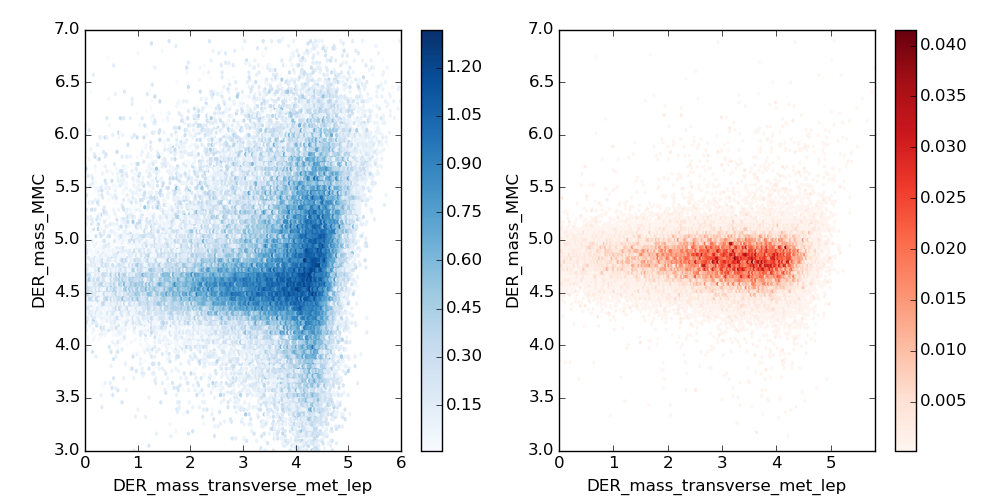
\includegraphics[scale=0.6]{scatter1.png}\\
\caption{\tiny{Background and Signal in 2d feature space}}
\end{figure}
\item In this project we propose a meta algorithm for the binary classification task and measure its performance through the AMS ($\sigma$) metric. 
\end{itemize}
\begin{minipage}{0.57\textwidth}
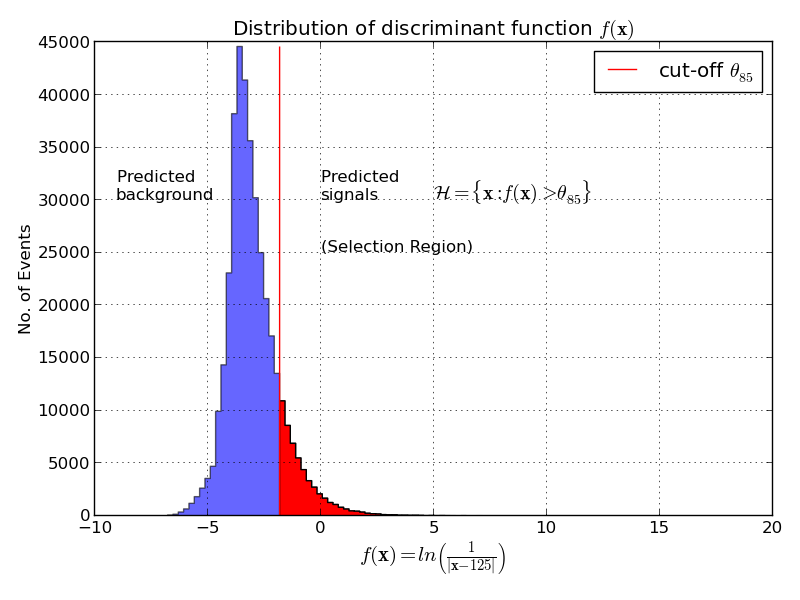
\includegraphics[width=\textwidth]{selection_region.png}
\end{minipage}
\begin{minipage}{0.3\textwidth}\raggedleft
\begin{equation*}
\scriptstyle{
\textrm{$AMS$} = \sqrt{2\bigg((s + b)\ln\bigg(1 + \frac{s}{b}\bigg)-s\bigg)} }
\end{equation*}
\raggedright The AMS is computed on the basis of events in the selection region of a classifier.
\end{minipage}
\end{block}

\begin{block}{Tree learning}
The primitive binary tree is constructed by applying axis-parallel splits on each feature until a stopping criterion is reached. This gives rectangular decision boundaries. When trees are combined these rectangular regions intersect giving more intricate boundaries.\\ \vspace{0.1cm}
\begin{minipage}{0.60\textwidth}
\begin{figure}
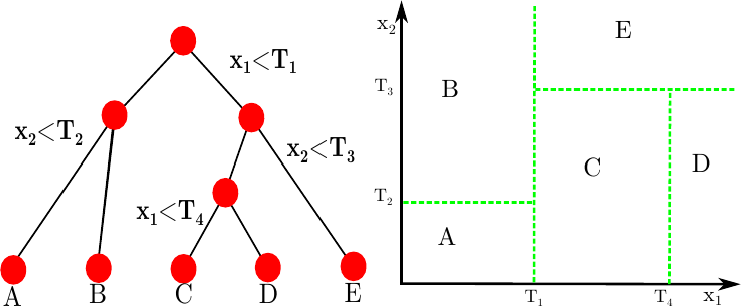
\includegraphics[width=\textwidth]{tree_learner.png}
\caption{\tiny{Depiction of the rudimentary tree learner in 2 features.}}
\end{figure}
\end{minipage}
\begin{minipage}{0.36\linewidth} \raggedright
The tree (left) has a depth of 4 and the nodes [A,$\ldots$,E] represent leaves, these might not be pure (i.e. contain samples of one class). All samples end up in a leaf and are assigned a score equal to the fraction of events of the same class in that leaf. 
\end{minipage} 

\begin{minipage}{0.36\linewidth} \raggedright
For example, if leaf $C$ has 30 background events and 2 signal events, the signal events in leaf $C$ will have a score of $1/16$ and background events will have a score of $15/16$. 
\end{minipage}
\begin{minipage}{0.6\linewidth}
\begin{figure}
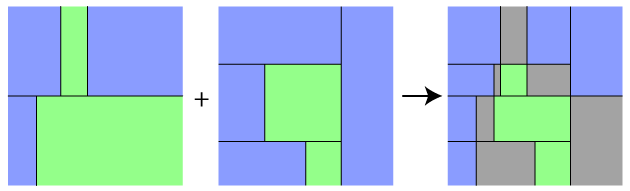
\includegraphics[width=\textwidth]{tree_boundary.png}
\caption{\tiny{Tree boundary of a 2 tree forest}}
\end{figure}
\end{minipage}

\end{block}

\end{textblock}

% Second column

\begin{textblock}{20}(21.2,6.3)

\begin{block}{Algorithm}

\begin{figure}
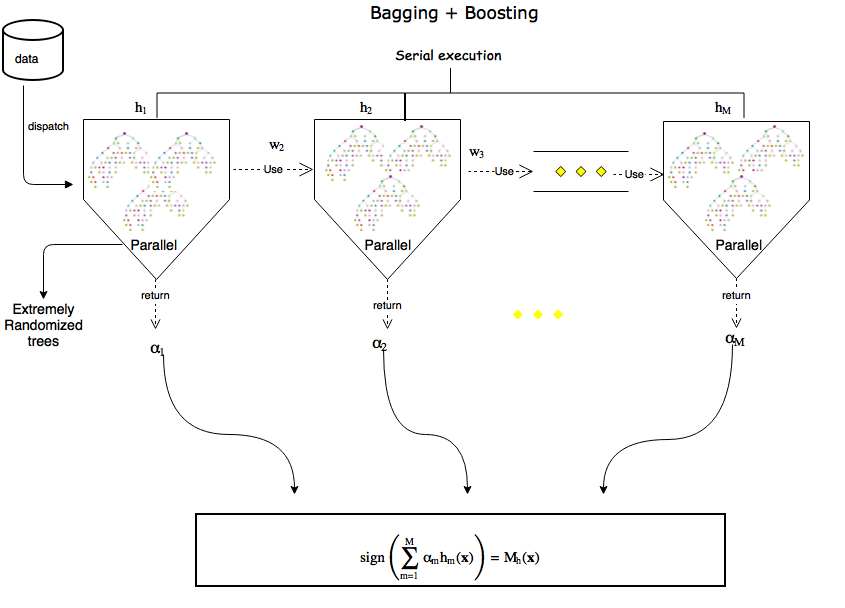
\includegraphics[scale=0.65]{bagboost.png}
\caption{\tiny{Meta-algorithm that combines bagging and boosting}}
\end{figure}
\vspace{-8mm}
\captionof{algorithm}{\tiny{Splitting algorithm used in extremely random trees}}
\begin{algorithmic}[1]
\STATE \textbf{Select} $K$ features ${x_{1}, \dots , x_{K}}$ at random from the training set $\mathbf{D}$.
\STATE \textbf{Select} $K$ splits $\{T_{1}, \dots , T_{K}\}$, one per feature for the $K$ features chosen in step 1; each $T_{i}$ is selected at random from the range of the feature values $\forall i = 1,\dots,K$.
\STATE \textbf{Rank} the splits $T_{i}$ by a criterion say $Q$ which gives a score $Q(\mathbf{D}, T_{i}) \in \mathbb{R}$ for each split. 
\STATE \textbf{Return} $T_{*} = max_{i=1 \dots K}Q(\mathbf{D}, T_{i})$.  
\end{algorithmic}
\end{block}

\begin{block}{Results}
\begin{figure}
\begin{minipage}{0.95\textwidth}
\centering
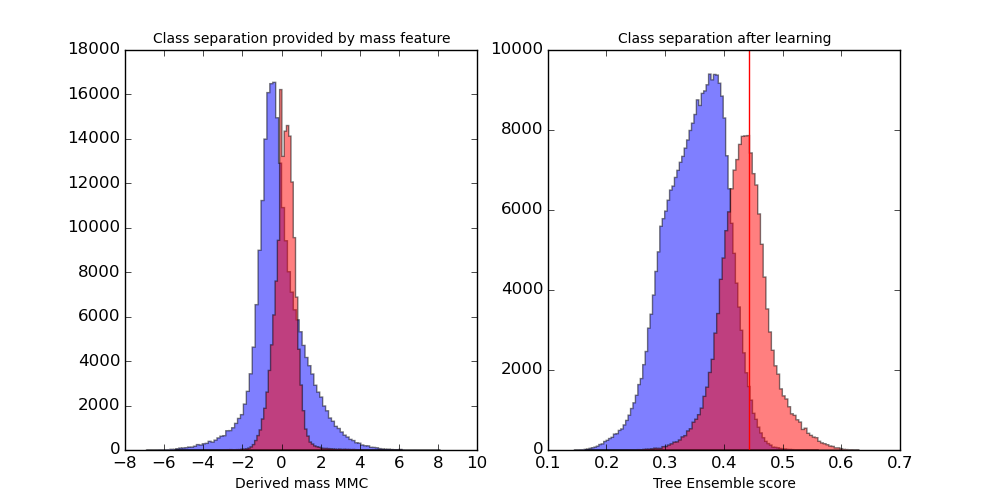
\includegraphics[scale=0.65]{separation.png}
\caption{\tiny{Signal and background separation provided by the mass feature (left) and by the tree ensemble score (right). The vertical line defines the selection region. We can notice superior separation post learning.}}
\end{minipage}
\end{figure}
\vspace{-8mm}
\begin{figure}
\begin{minipage}{0.95\textwidth}
\centering
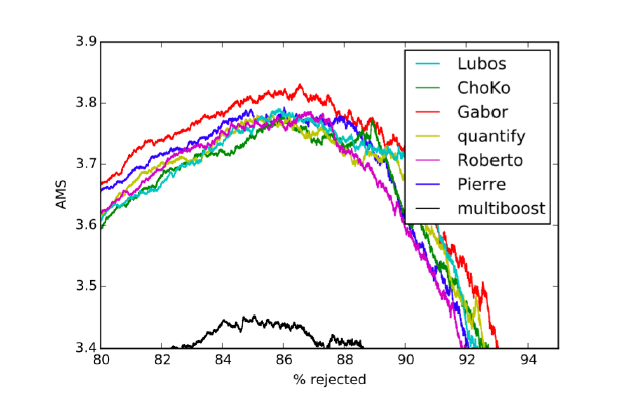
\includegraphics[width=0.5\linewidth, height=203pt]{WinningAMS.png}
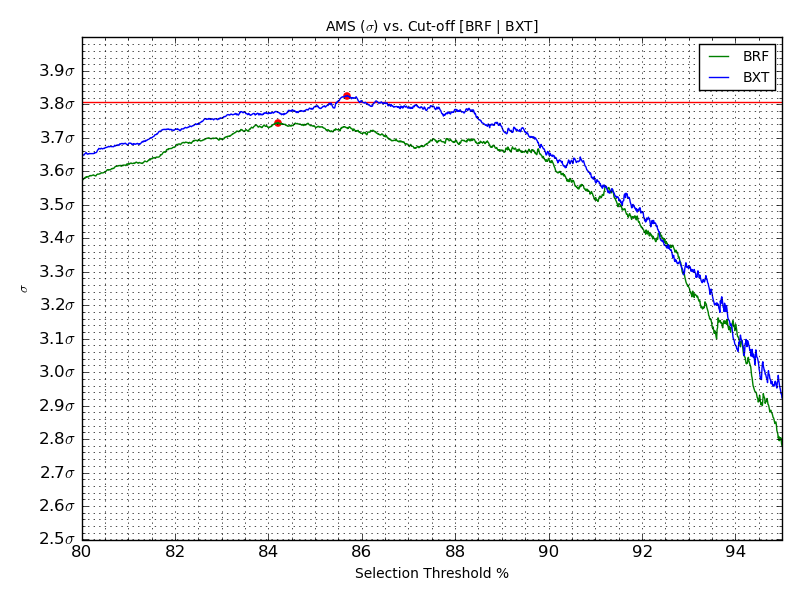
\includegraphics[width=0.5\linewidth]{AMS_Curve_BXT_BRF.png}
\caption{\tiny{Leading solutions for the ATLAS Higgs classification (left) and the proposed algorithm (right) which uses a boosted version of tree ensembles. The green curve shows the significance curve obtained by boosting traditional forests (BRF) and the blue curve is obtained by boosting extremely random trees (BXT).}} %At the 85$\%$ cut-off the proposed algorithm has a score of 3.7936, the best solution (bagged neural networks) at that cut-off has a score of 3.8058 (Gabor).}}
\end{minipage}
\end{figure}
\end{block}
\vspace{-6mm}

\begin{block}{References}
\begin{minipage}{0.9\linewidth}
     {
     \printbibliography
     } 
\end{minipage}
%\vspace{2ex}
\end{block}

\end{textblock}

\end{frame}
\end{document}
